\documentclass[english]{uzhpub}
\usepackage[T1]{fontenc}
\usepackage[latin9]{inputenc}
\usepackage{url}
\usepackage{hyperref}
\usepackage{epstopdf}
\usepackage[round,comma]{natbib}
\interfootnotelinepenalty=10000
\bibliographystyle{abbrvnat}

\hypersetup{
    colorlinks=true,
    linkcolor=black,
    filecolor=black,      
    urlcolor=black,
    citecolor=black
}

\renewcommand{\baselinestretch}{1.5}

\begin{document}

%% Titelei
\title{Scale-Invariant Export Contents from I/O-Tables}

%\subtitle{}

\author{Luzius Meisser, luzius@meissereconomics.com}

\date{2016-04-19}

\maketitle

%\emph{The Leontief inverse is the standard tool to calculate the import content of exports (also known as import reuse, foreign contents of exports, foreign value added and vertical specialization) from given input-output tables. Unfortunately, it only yields correct results when the inputs are proportionally used for the production of the outputs in each sector, which rarely is the case. As a consequence, input reuse as calculated by the Leontief inverse depends on the resolution of the underlying data. In case of the WIOD dataset, global average import reuse climbs steadily from 17\% to 24\% as the resolution is increased from one to thirty-five sectors per country. I address this known problem by postulating a hidden variable 'domestic consumption preference' to construct a scale-invariant computation method, resulting in a more credible -- but maybe still too low -- value of 32\% globally.}

\emph{The Leontief inverse is the standard tool to calculate the import content of exports from given input-output tables. Unfortunately, it only yields correct results when inputs are proportionally used for the production of outputs, which rarely is the case. As a consequence, the value calculated by the Leontief inverse depends on the resolution of the underlying data. With the WIOD dataset, global import contents of exports climb from 17\% to 24\% as the resolution is increased from one to thirty-five sectors per country. I address this known problem by constructing a new, scale-invariant computation method, resulting in more credible 32\%.}

\section{Introduction}
% The OECD refers to import reuse as \href{http://www.oecd-ilibrary.org/trade/data/oecd-wto-statistics-on-trade-in-value-added_data-00648-en}{foreign value added share of gross exports}  Sometimes, the term "import contents of exports" (e.g. http://www.wiod.org/publications/papers/wiod5.pdf), but not consistently across different sources (OECD differs).
Import reuse (also known as import content of exports, foreign contents of exports, foreign value added share of gross exports, foreign value added and vertical specialization \cite{hummels2001nature})\footnote{These terms are not always used consistently and do not always refer to the same metric. However, all of them suffer from the same problem when calculated with the Leontief inverse.} is a basic metric that is typically derived from input-output tables and often serves as an intermediate step for more elaborate calculations, for example as a contributing factor when estimating exchange-rate pass-through. It measures the extent to which exports consist of previous imports. Its usual method of calculation is to derive the composition of exports by applying the Leontief inverse to the input-output table of the exporting country. More accurate results are achieved when basing the calculation on a worldwide input-output table such as WIOD, as this allows to account for circular flows of goods between countries. \citep{auer2016international}

The known problem with this traditional approach is that the Leontief inverse implicitly assumes proportional use of inputs. In practice, however, firms that import much also tend to export much. \ref{Amiti} When aggregating such firms together with firms that have low import intensity, information about the actual use of specific imports gets lost and the import reuse as calculated by the Leontief inverse decreases. Thus, when the import intensity and the export intensity of sectors beyond the resolution of the data at hand are positively correlated, the Leontief inverse systematically underestimates import reuse. This effect was already observed in 1991 by Mark Planting who compared using 6800 versus 536 sectors, which is why the OECD considers the Leontief result a "conservative indicator of the actual input activity". \citep{oecd2000}

\cite{koopman2012tracing} as well as \cite{kee2013domestic}, both focusing on China, address this problem by enriching input-output tables with additional data to isolate processing trade. Koopman et al. summarize their approach as follows: "The basic idea is to use information from the standard I/O table to determine sector-level total imports/exports, and information from trade statistics to determine the relative proportion of processing and normal exports within each sector." Similarly to the findings presented in here, they find that actual import reuse is much higher than what the traditional described by \cite{hummels2001nature} suggests. In contrast to these previous approaches, I present a method to better estimate import reuse that does not rely on having additional data, but instead calculates a more plausible result from input-output tables alone under the assumption of self-similarity.

Generally, I treat economic trade flows as a graph and not as a matrix, a choice motivated in section \ref{sec:data}, which also describes the used data more closely. Section \ref{sec:method} specifies the applied methods, in particular how the introduction a hidden variable \emph{domestic consumption preference} allows the calculated import reuse to be tuned such that it becomes robust against changes in resolution (scale-invariant). This is followed by results section \ref{sec:result}, that presents selected findings, and a concluding section \ref{sec:conclusion}. All source code, input data, and outputs can be found on \href{https://github.com/kronrod/importreuse}{github.com/kronrod/importreuse}.

\section{Data}
\label{sec:data}
\subsection{WIOD}
The world input-output database (WIOD) presented by \cite{timmer2012world} serves as data source. It covers 42 countries and 17 years starting from 1995 with a resolution of 40 sectors per country. Unlike national input-output tables, the WIOD tables contain disaggregate flows between the individual sectors of different country. Furthermore, it does not depend as strongly on the proportionality assumption as other data sources, merely using it within use categories.
%http://www.wiod.org/publications/source_docs/WIOD_sources.pdf

For simplicity, I merge each country's destination sectors such as consumption and inventory changes into one node "consumption and capital formation" that is treated specially and generally not counted as a sector. I.e., when later reducing the number of sectors per country to one, there will actually be two nodes left per country, one active sector and the consumption node. Furthermore, I ignore negative flows into the consumption node\footnote{This can happen when capital is reduced or inventories decrease.} as they are negligible and not having negative edge weights is a prerequisite for the later applied Edmonds-Karp algorithm \cite{edmonds1972theoretical}. All other flows in WIOD are zero or positive.

\subsection{Graph View}
\label{sec:graphview}
Usually, economists treat input-output tables as matrices. An equally valid and in this case more insightful view is to treat the input-output table as a weighted directed graph. Every square matrix can be represented as a weighted directed graph and a weighted directed graph can converted into a square matrix as long as there is at most one edge in each direction between each pair of nodes. In the graph representation of input-output tables, each node represents a sector in a country and is named accordingly. Each weighted edge $e=(a, b, w)$ represents a flow from node $a$ to node $b$ of volume or weight $w$. Flows from a node to itself are allowed and correspond to diagonal elements in the matrix view.

When merging two nodes $a$ and $b$ of a graph into a new node $c$, the nodes $a$ and $b$ are replaced by $c$ in all edges and then all edges that connect the same nodes in the same direction aggregated into a single new edge whose weight is the sum of the old weights. This is equivalent to first removing column $i$ and adding it to column $j$ in the matrix view, and then also removing row $i$ and adding it to row $j$, with $i$ and $j$ being the indices of the two sectors represented by nodes $a$ and $b$. When doing so, the indices of other sectors may change, making it less convenient to track a specific sector in the matrix view than in the graph view, where the names of unaffected nodes stay the same when others are merged. Generally, the graph view is more compact than the matrix view when the matrix is sparse.

\section{Method}
\label{sec:method}

\subsection{Varying the Sector Resolution}
\label{Varying}
The usual method to calculate input reuse is to apply the Leontief inverse to the input-output table. A known flaw of this approach is that it implicitly assumes proportional use of inputs.\footnote{This is \emph{not} what is usually called the proportionality assumption. The proportionality assumption in the context of input-output analysis usually means proportionally assigning an import like steel across the domestic sectors that use that import. Here, proportional use of inputs refers to proportionally assigning the inputs of a single sector to its outputs. To avoid confusion, I refer to the latter as \emph{proportional assignment}.} This should not be a problem for disaggregate data with atomic resolution, but when applied to aggregate data, the Leontief inverse is systematically biased with countries that prefer consuming domestic products over foreign products. The import reuse as calculated by the Leontief inverse usually grows as the resolution of the underlying data is increased, which is a strong hint that it cannot be trusted. In case of the WIOD data, world input reuse grows from 17\% to 24\% as the resolution is varied between one and thirty-five sectors, a result discussed in section \ref{res:varying}. Thus, the Leontief inverse is not scale-invariant. A scale-invariant computation method that is consistent across different resolutions would yield more credible results, which is exactly what will be constructed in the subsequent sections.

\subsection{Maximum Flow}
Given the input-output graph of a country, one can derive the minimum and maximum possible import reuse by computing the maximum amount of imports that can be directed towards domestic consumption (for the minimum) or towards foreign nodes as exports (for the maximum). This problem is known as the \emph{maximum flow problem} and can for example be solved with the Edmonds-Karp algorithm. \cite{edmonds1972theoretical} The true import reuse must lay within the calculated bounds, with the proportional variant being somewhere in between. Unfortunately, these bounds turn out to be so wide that they cannot provide much guidance as to where the true import reuse might be.

\subsection{Domestic Consumption Preference}
To seek for plausible values of import reuse within the given bounds, I introduce a parameter \emph{domestic consumption preference} $p_{dom} \in [0,1]$. It is defined as the fraction of domestic inputs of a sector that directly flows into domestic consumption, before proportionally distributing all the remaining flows.\footnote{To be more precise, the direct flow from sector $s$ to the consumption node before proportionally distributing the remaining flows is $max(w_{s,c}, p_{dom} (v_s + i_{dom,s}))$, with $w_{s,c}$ being the weight of the edge connecting $s$ to the consumption node $c$, $v_s$ being value creation of $s$, and $i_{dom,s}$ being the total value of the domestic inputs of $s$. As a prerequisite for calculating $i_{dom,s}$, the import contents of all inputs of $s$ must be known.} For example, if there are two firms in the beer sector of a country, one producing beer from domestic hops and one producing beer from imported hops, a positive domestic consumption preference indicates that the locals prefer to drink the former and export the latter, whereas the proportional assignment implies indifference.

By exogenously varying $p_{dom}$, an interval of potential true values of import reuse can be explored, with $p_{dom}=0$ corresponding to the proportional assignment, and $p_{dom}=1$ being somewhere between the proportional result and the maximum flow result. It does not quite reach the maximum as merely redirecting the domestic flows of every node towards local consumption is not sufficient. In some cases, it is necessary to redirect locally created value through multiple nodes towards consumption, which is what maximum flow implies, but not $p_{dom}=1$ as defined above. In future research, it might be desirable to redefine domestic consumption preference such that it can cover the whole range given by the bounds of maximum flow, including negative values that would correspond to a preference for foreign goods. In the data at hand, this actually seems to be the case for Russia in some years. But for the time being, the definition at hand is broad enough.

\subsection{Scale-Invariance}
\label{met:scale-invariance}
Equipped with a parameter to tune, one can try to find values of $p_{dom}$ that make the calculate import reuse scale-invariant. One can do this globally with one global $p_{dom}$, or nationally with a separate domestic consumption preference $p_{dom,c}$ for each country $c$. In both cases, the parameter is adjusted such that the covariance $cov(r, f)$ of resolution $r$ (the number of sectors per country) and resulting import reuse $f$ is minimized. I calculate these values iteratively simply by updating import contents in the worldwide input-output graph until the values stabilize.\footnote{This is done in script \href{https://github.com/kronrod/importreuse/blob/master/src/com/meissereconomics/seminar/run/BendingByCountry.java}{BendingByCountry}.}

Being robust against the tested changes in resolution, the import reuse resulting from assuming the scale-invariant domestic consumption preference is more plausible than the one calculated with the proportional assignment of inputs. Under the assumption that it is also robust against changes in resolution beyond the limits of the data at hand, the calculated scale-invariant import reuse matches the true import reuse. This assumption is valid if the input-output graph is self-similar, i.e. if the network similarly structured at all scales. Given that a wide range of real-world networks exhibit self-similarity \cite{song2005self}, this might be the best possible estimate in the absence of more fine-grained data.

\section{Result}
\label{sec:result}

\subsection{Varying the Resolution}
\label{res:varying}

Figure \ref{fig:varying} shows how the global import reuse calculated with the traditional method of applying the Leontief inverse depends on the resolution of the underlying data.\footnote{The raw data for this figure has been generated with script \href{https://github.com/kronrod/importreuse/blob/master/src/com/meissereconomics/seminar/run/Figure1Resolution.java}{Figure1Resolution}.} As the number of sectors is increased from one to the thirty-five, import reuse continuously climbs from 17\% to 24\%. This is a clear signal that the true global import reuse is higher than what is typically assumed.

\begin{figure}
\centering
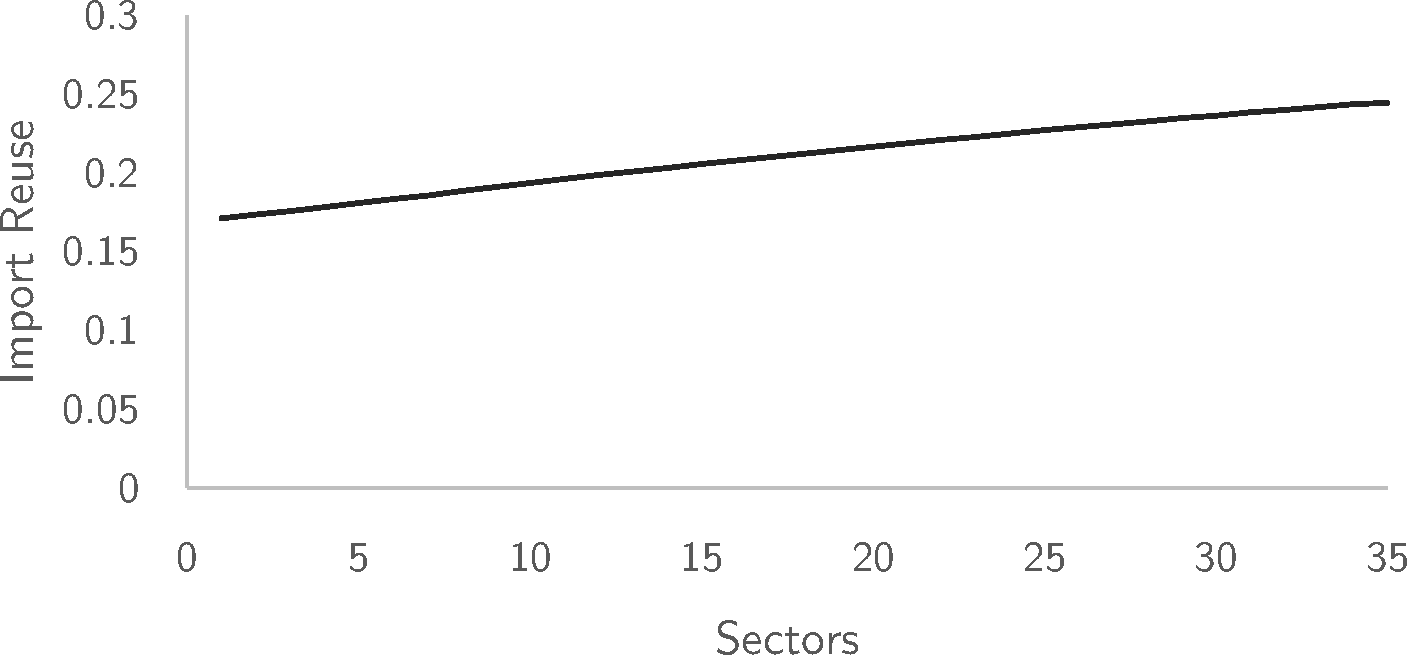
\includegraphics[scale=0.4]{../data/resolution}
\caption{The calculated import reuse depends on the resolution of the underlying data. The plotted curve represents the average of 100 randomized runs and uses the data of 2005. The standard deviation of each plotted point is less than $10^{-5}$, so the curve can be considered free from visible random variation.} \label{fig:varying}
\end{figure}

The program to calculate the data behind figure \ref{fig:varying} first parses the given world input-output table into a graph, and then repeatedly calculates import reuse and reduces the number of sectors in each country by one. This is done by randomly selecting two sectors in each country and merging them as defined in section \ref{sec:graphview}. The reported import reuse is a global volume-weighted average of the import content of all exports, which in turn are calculated by repeatedly updating the input composition of each node until all values have converged towards a stable equilibrium. This latter step equivalent to applying the Leontief inverse to the matrix view.

When plotting the same curve for the 40 available countries individually, results vary, but all except Russia's import reuse raises as the resolution increases. For Russia, the curve slightly declines, at least for some of the years in the dataset, indicating that the domestic input preference of Russia is slightly negative.

\subsection{Scale-Invariance}
As a next step, domestic consumption preference $p_{dom}$ is varied as described in section \ref{met:scale-invariance}. Figure \ref{fig:germany} shows how the slope of Germany's reuse-resolution curve changes as $p_{dom}$ is varied. For $p_{dom}=XXX$ it is flat, with $cov(r, f) = 0.0001 XXX$. Depending on the country, the scale-invariant value of $p_{dom}$ varies. Also, it varies over time. Figure \ref{fig:time} shows how Greece's import reuse and domestic consumption preferences changed over time. Both variables have comparable variances over time. TODO: figure with traditional and new import reuse, plus preference for Greece.

Table \ref{tab:ranking} ranks countries by domestic consumption preference of 2011. The raw data for all other years and other countries for the aforementioned figures can be found in file href{asdasd}{XXX}. It is unclear whether much meaning should be attributed to this hidden variable, and if so, what it it should be exactly. Is there a pattern behind the countries with low domestic consumption preference? This might be an interesting question for future research.

\subsection{Drivers of Import Reuse}
Import reuse varies across countries. The most important driver of import reuse is the import volume relative to the country's economy, here measured as import share $s = imports / (consumption + exports)$. Import share $s_{c,y}$ of a country $c$ in year $y$ can already explain 72\% of import reuse $f_{c,y}$. Together with domestic consumption preference $p_{dom,c,y}$, the $R^2$ is improved to 92\% when regressing:

\[f_{c,y} = b_0 + b_1 s_{c,y} + b_2 p_{dom,c,y}\]

Both variables are highly significant (t-stat above 40). Given that $p_{dom,c,y}$ is the variable used for mininizing $corr(f_c, r)$ in each year, this is not surprising. However, $p_{dom,c,y}$ even has significant explanatory power for the traditional Leontief import reuse (t-stat 17.58). All the underlying data is available as \href{https://github.com/kronrod/importreuse/blob/master/data/reusedrivers.dta}{reusedrivers.dta} and \href{https://github.com/kronrod/importreuse/blob/master/data/reusedrivers.dta}{reusedrivers.csv}, and the stata output as \href{https://github.com/kronrod/importreuse/blob/master/data/reusedrivers.pdf}{reusedrivers.pdf}.

\section{Conclusion}
\label{sec:conclusion}
I demonstrated that the standard approach of calculating input reuse from input-output tables strongly depends on the resolution of the underlying data and thus cannot be trusted when applied to the highly aggregate data usually provided by input-output tables. To address this flaw, I postulate a hidden variable \emph{domestic consumption preference} for each country and year, and tune it such that the calculated import reuse becomes scale-invariant, thereby fixing the aforementioned flaw. Assuming that input-output tables stay self-similar when increasing their resolution beyond the resolution of the available data, this improved approach yields the true import reuse.

When applied to atomic data,\footnote{A hypothetical input-output table with atomic resolution would allow to track the exact trade path of every single apple as well as every other good at its atomic quantity.} all discussed approaches must yield the same result, as they must stay within the bounds given by maximum flow, which converge towards the true import reuse as the resolution is increased. In theory, any value within these bounds could be the true value and the slope of the curve shown in figure \ref{fig:resolution} could change multiple times in all conceivable directions when the resolution is further increased. However, in absence of evidence to the contrary, the simplest assumption should be considered the most probable, namely that the structure of the data remains roughly the same at smaller scales. In that case, the scale-invariant estimate is the best guess for the true import reuse.

The presented approach raises the important question whether the introduced hidden variable \emph{domestic consumption preference} is purely technical or whether it has broader implications. Deriving and testing such implications could constitute worthwhile future research. But first, one should verify whether this proposed approach yields consistent results when applied to other, and in particular more fine-grained data. Also, one could dig deeper into the specific ways in which the input-output graph must be self-similar in order for the results to be robust. A related question is whether the assumption taken for the construction of the input-output tables (for example the proportionality assumption) causes systemic distortions. Lastly, it would also be nice to improve algorithmic elegance and computational efficiency.

\bibliography{termpaper}

\end{document}
